\chapter{Funktionsweise von Spark}
\label{chapter:funktionsweise von Spark}


Im vohergehenden Kapitel wurde der Berkeley Data Analytics Stack vorgestellt. Es wurde gezeigt, dass dieser aus einer Reihe von Bibliotheken, Infrastrukturkomponenten und dem eigentlich Kern, Apache Spark, besteht.

In diesem Kapitel werden die grundlegenden Konzepte von Spark vorgestellt und dessen Funktionsweise betrachtet. Einleitend wird gezeigt, wie eine Spark-Infrastruktur aufgebaut sein kann, wie diese intern Abfragen und eigene Spark-Programme verarbeitet und wie der \textit{Spark-Context} sich als Cluster-Repräsentant gegenüber dem Anwender und der API exponiert. Im nächsten Unterkapitel wird die eigentliche Basis von Apache Spark vorgestellt. Spark basiert im Wesentlichen auf einer verteilten Datenstruktur, den \textit{Resilient Distributed Datasets}. Deren Konzept wird sowohl theoretisch, als auch im Anwendungskontext dargestellt. 

Ein weiteres Kernelement der Spark-Implementierung bildet das \textit{In-Memory-Processing} der Daten. Spark ist in der Lage, je nach Konfiguration des Host-Systems, große Teile der Analysen und Verarbeitungen äußerst flexibel im Hauptspeicher durchzuführen und so massive Performanceverbesserungen gegenüber festspeicherbasierter Verarbeitung zu generieren. Hierzu bietet Spark spezielle \textit{In-Memory-Primitives} an. In einem weiteren Unterkapitel werden dieses detailliert vorgestellt. 



\section{Spark im Cluster}
\label{section:spark im cluster}

%Diesen Abschnitt noch mit Referenzen untermauern
Eine große Herausforderung im Umfeld verteilter und nebenläufiger Analyse und Verarbeitung großer Datenmengen stellt der Netzwerkverkehr da. Der klassische Aufbau einer verteilten Anwendung hält die Daten auf einer dafür vorgesehen Plattform im Netzwerk. Häufig ist dies ein dedizierter File- oder Datenbankserver, der mit möglichst großer Bandbreite mit dem Applikationsserver verbunden ist. 

%Hier muss noch eine Grafik eines herkömmlichen Netzwerks rein
\begin{figure}[htb!]
\centering
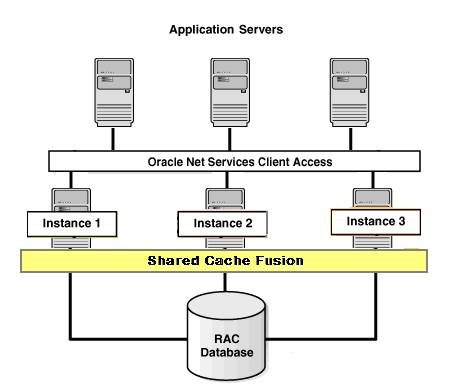
\includegraphics[width=1.0\textwidth]{bilder/oracle_cluster.jpg}
\caption{Aufbau eines Standardcluster im Rechenzentrumsbetrieb mit Application-Server und Oracle Datenbanken \protect\citeint{or14}. }
\label{fig:oracle}
\end{figure} 

In Abbildung \ref{fig:oracle} wird ein möglicher Aufbau eines herkömmlichen Clusters gezeigt. Dieser besteht in diesem Fall aus drei Applikationsservern, die wiederum über drei Instanzen eines verteilten Caching-Systems auf eine zentrale Datenbank zugreifen. In einem solchen Aufbau entsteht in der Regel eine sehr hohe Netzwerklast, da die für die Applikation benötigten Daten dieser zunächst zur Verfügung gestellt werden müssen. Die Applikation fragt die Daten ab, diese werden dann von der Datenbank zu den Applikationsservern geliefert, hier meist in Applikationsobjekte umgewandelt und stehen dann der Anwendung zur Verfügung. 

Spark geht hier einen anderen Weg. Ein Spark-Cluster besteht typischerweise aus einem zentralen \textit{Master} und n \textit{Worker-Nodes}. Diese können aus einfachen Servern bestehen, aber auch aus Clustern von Mainframes (beispielsweise IBM Z, Oracle ExaLogic, etc.). Das Hadoop Distributed File System und Spark skalieren über Cluster beliebiger Größenordnung. Über ein verteiltes Dateisystem werden die Daten auf dem Cluster gehalten und sowohl dem \textit{Master}, als auch den \textit{Worker-Nodes} so zur Verfügung gestellt. 

%Hier Grafik zum Aufbau eines Spark Clusters. 
\begin{figure}[htb!]
\centering
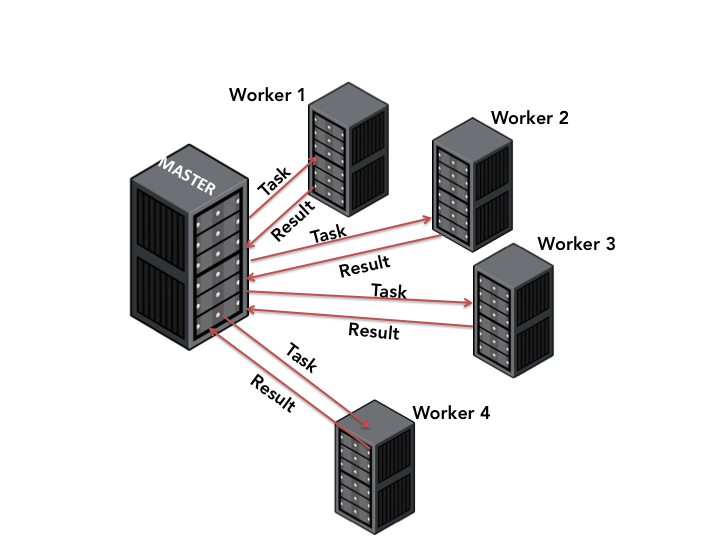
\includegraphics[width=1.0\textwidth]{bilder/spark1.png}
\caption{Clusteraufbau mit Spark mit einem Master und vier Worker-Nodes. }
\label{fig:sparkclustermastermitworker}
\end{figure} 



Abblildung \ref{fig:sparkclustermastermitworker} zeigt den Aufbau eines Spark-Clusters. Spark-Anwendungen laufen als unabhängiges Set von Prozessen auf Cluster-Infrastrukturen. Das Hauptprogramm, der sogenannte \textit{Spark Driver}, instanziert das\textit{ SparkContext-Objekt}, das die einzelnen Prozesse koordiniert. Auf Clustersystemen hält der \textit{SparkContext} die Verbindung zum jeweiligen \textit{Cluster-Ressource-Manager} (Mesos, Yarn), im Standalone-Betrieb instanziert der Context selbst einen Dummy-Manager und allokiert in beiden Fällen die für die Anwendung nötigen Hardware-Ressourcen. Die Cluster-Manager liefern ihren aktuellen Status an Spark zurück und melden Auslastung und Gesundheitszustand der einzelnen Knoten. Über interne \textit{Load-Balancing-Systeme}\footnote{Load-Balancing-Systeme sind Überwachungsmechanismen in verteilten Systemen. Jedes Teilsystem meldet seine eigene Auslastung und seine Verfügbarkeit an den Load-Balancer. Dieser verteilt anstehenden Aufgaben so auf die Ressourcen, dass eine möglichst gleichmäßige Verteilung über die gesamte Infrastruktur möglich ist.} wird ermittelt, welche Worker-Nodes die jeweiligen Tasks aus dem Spark-Kontext zugewiesen bekommen. Der SparkContext repräsentiert sowohl für die Spark-Konsole REPL, als auch in eigenen Spark-Programmen innerhalb der APIs das gesamte Cluster. Dem SparkContext wird bei der Initialisierung über ein Konfigurationsobjekt mitgeteilt, welche Ressourcen ihm für das aktuelle Programm zur Verfügung stehen. Die Entscheidung, welche, der initial zur Verfügung gestellten Nodes oder Ressourcen des Clusters von Spark wann in Anspruch genommen werden, obliegt der Kombination aus Spark und \textit{Cluster-Ressource-Manager}. 

%gesamten Abschnitt mit Referenzen belegen!    

%fußnote nochmal überdenken

\begin{figure}[htb!]
\centering
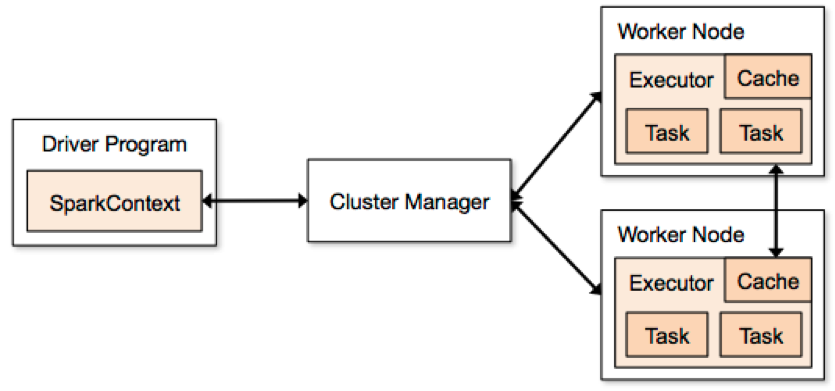
\includegraphics[width=1.0\textwidth]{bilder/3_2_cluster.png}
\caption{Clusteraufbau mit Spark \protect\citeint{sp14}}
\label{fig:sparkcluster}
\end{figure} 





Wenn ein SparkContext initialisiert wurde, installiert der Spark sogenannte \textit{Executors} auf sämtlichen Worker-Nodes des Clusters. Der Applikationscode wird nun als JAR\footnote{Ein JAR (Java ARchive) ist ein gepacktes und auf einer Java Virtual Machine ausführbares (Java, Scala, Clojure) Programmpaket, häufig inklusive der benötigten Bibliotheken.} direkt an die Executors verteilt und dieser anschließend durch entsprechende Tasks ausgeführt. 



  
\section{Das Konzept der Resilient Distributed Datasets}
\label{section:rdd}

Die Resiliient Distributed Datasets (RDD) sind das eigentliche Kernelement von Apache Spark. Hierbei handelt es sich um fehlertolerante, parallele Datenstrukturen, die dem Anwender erlauben, Zwischenergebnisse explizit im Hauptspeicher zu halten, ihre Partitionierung zu steuern, um Daten bewusst an bestimmten Stellen halten zu können und diese mittels umfangreichen Operatoren zu manipulieren  \citelit{rdd12}. Das Konzept der RDDs entspricht prinzipiell den Views\footnote{Eine View ist in einem relationalen Datenbanksystem die Ergebnismenge einer persistierten Datenbankabfrage auf bestimmte Daten. Diese lässt Abfragen analog zu einer gewöhnlichen Tabelle zu.} in relationalen Datenbanksystemen. Werden die RDDs für weitere Zugriffe persistiert, entspricht dies dem Prinzip der Materialized Views\footnote{Materialized Views entsprechen bei Abfragen den regulären Views. Allerdings wird hier im Gegensatz zu den Views bei Zugriff keine Abfrage auf die zugrundeliegenden Tabellen durchgeführt. Stattdessen sind die Daten als Kopie in eigenen Datenbankobjekten persistent vorhanden.}.  

RDDs werden mittels deterministischer, paralleler Operationen erstellt, den sogenannten \textit{Transformationen}. Im Fehlerfall, also wenn beispielsweise ein \textit{Node} im Cluster ausfällt, können die RDDs automatisch anhand der durchgeführten Regeln neu aufgebaut werden. Deshalb merken sich die RDDs die Transformationen, die zu ihrem Aufbau geführt haben und können so verlorene Datenstrukturen schnell rekonstruieren. Die \textit{Resilient Distributed Datasets} können ausschließlich durch Transformationen, wie beispielsweise \textit{map, filter, join}, etc., auf Daten aus dem Dateisystem oder aus anderen, bereits vorhandenen RDDs erzeugt werden, oder durch Verteilen einer Object-Collection in der Driver-Applikation. Diese Datenstrukturen müssen nicht persistiert werden, da sie für einen Partitionierung ausreichende Informationen über ihre Erstellungsregeln und die entsprechenden Datensätze enthalten, das sogenannte \textit{Lineage} \citelit{rdd12}.   

Da es sich bei RDDs prinzipiell um Scala-Collections handelt, können diese auch direkt in Scala-Code eingebunden und verarbeitet werden, oder interaktiv über die Scala-Konsole REPL genutzt werden. Aber auch für Java und Python bietet Spark APIs an. Für weitere Sprachen wie R oder Clojure existieren Wrapper-Frameworks, welche die RDDs und ihre Operationen verfügbar machen (Vergleich \ref{section:APIs}. RDDs können nur durch grobgranulare, deterministische Transformationen, erstellt werden \citelit{dz14}. 

WIe eingangs beschrieben, verfügen die Anwender von Spark über die Kontrolle der Aspekte \textit{Persistence} und \textit{Partitioning} \citelit{rdd12}. Mit der Persistence lässt sich festlegen, welche RDDs wiederverwendet werden sollen, also welche RDDs nach welcher Strategie persistiert werden. Dies ist besonders wichtig, da nicht explizit persistierte RDDs bei jeder darauf ausgeführten Operation neu berechnet werden. Das Partitioning legt fest, nach welchen Kriterien die RDDs geteilt und über das Cluster verteilt werden sollen, also beispielsweise sortiert nach bestimmten Keys. Die Optimierung der Partitionierung ist unter anderem elementar für Join-Operationen. Je nach Partitionierungsstrategie kann dies erhebliche Unterschiede in Laufzeit und Ressourcennutzung bedeuten \citelit{ls15}.  

RDDs können prinzipiell auf folgende Arten für die Wiederverwendung gespeichert werden \citeint{sp14}:
\begin{itemize}
		\item Als deserialisiertes Java-Objekt im Speicher der JVM – dieses Variante bietet die beste Performance, da die Objekte sich direkt im JVM-Heap befinden, benötigt jedoch aufgrund der \textit{Lazy Evaluation} ab dem Zeitpunkt der ersten Zugriffe Platz im Heap-Speicher der Laufzeitumgebung und können umfangreicher sein, als nötig. 
		\item Als serialisiertes Java-Objekt direkt im Speicher – dieses Verfahren ist effizienter bezüglich der Hauptspeicherauslastung da andere Speicherbereiche, als der JVM-Heap für die Materialisierung verwendet werden, aber schlechter in der Zugriffsgeschwindigkeit.
		\item Im Dateisystem – diese Variante ist erwartungsgemäß die langsamste, jedoch nötig, wenn die RDDs zu groß für die Haltung im RAM sind. 		
\end{itemize}	

Die Default-Serialisierung findet über die Java Standardbibliothek \texttt{ObjectOutputStream} für Serialisierung statt. So kann jede Klasse, die \texttt{java.io.Serializable} implementiert, serialisiert werden. Dies ist laut  \citeint{rdd12} oft nicht optimal, da dieser Serialisierer verhältnismäßig langsam ist und häufig zu sehr großen Serialisierungen führt. Spark bietet deshalb als Alternative den Kryo-Serialisierer an (Vergleich \citeint{kry14}). Dieser ist erheblich schneller und erstellt kompaktere Serialisierungen, als die Default-Implementierung. Nachteilig wirkt sich allerdings aus, dass nicht nicht alle Typen von Serialisierungen unterstützt werden und sämtliche zu serialisierenden Klassen bereits im Voraus registriert werden müssen. Gemäß \citeint{rdd12} wird der Einsatz des Kryo-Serialisierers insbesondere für netzwerkintensive Aufgaben mit Spark ausdrücklich empfohlen. 

  

\begin{figure}[htb!]
\centering
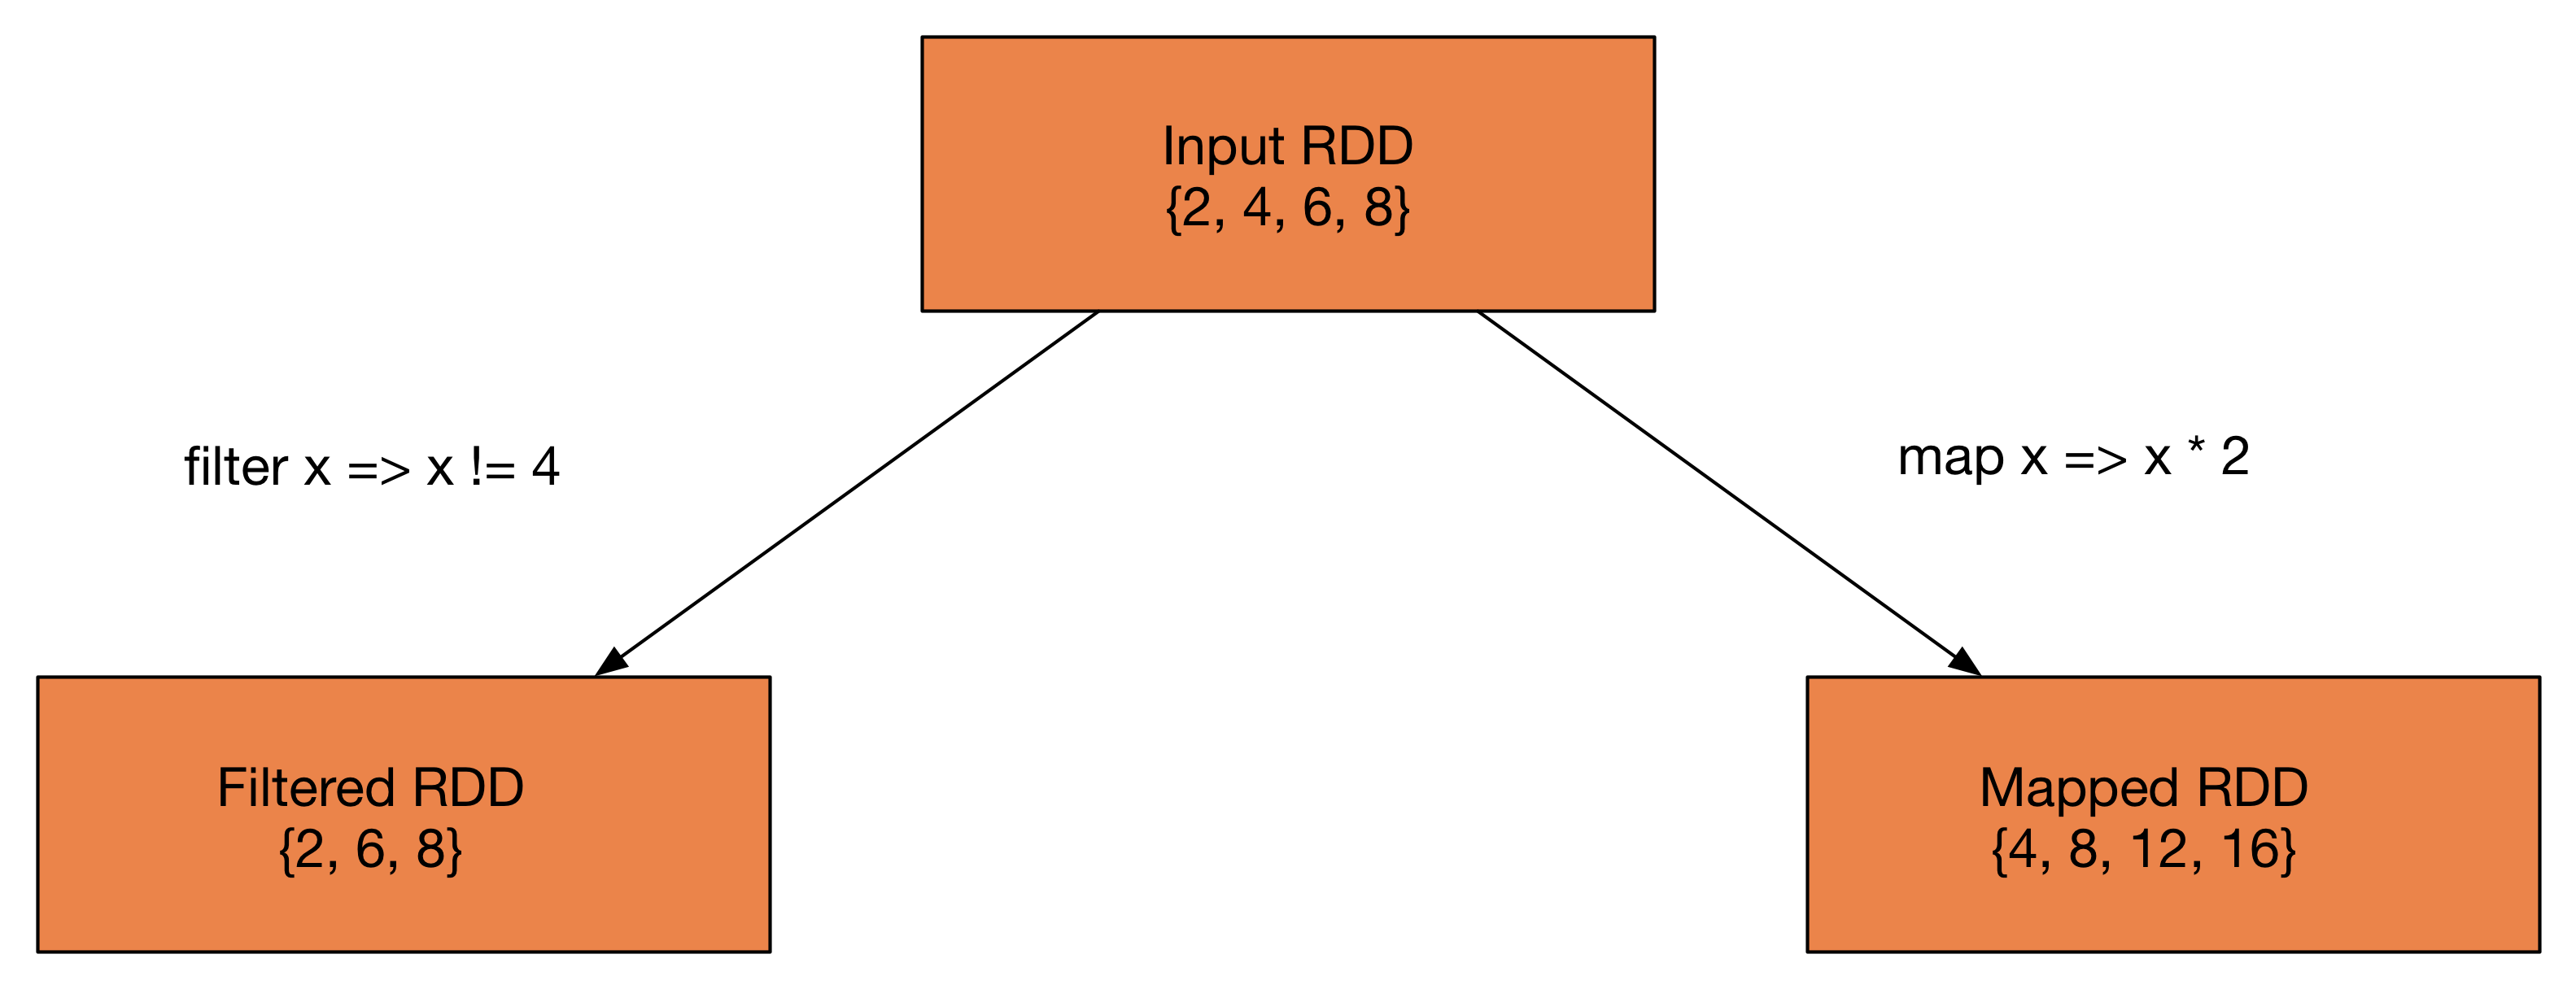
\includegraphics[width=1.0\textwidth]{bilder/transform.png}
\caption{Transformation von RDDs in Spark.}
\label{fig:sparktransform}
\end{figure} 



In der folgenden Tabelle befindet sich exemplarisch eine Auswahl\footnote{Die vollständige Übersicht über die Transformationen und Actions auf RDDs befindet sich im Anhang dieser Ausarbeitung.} der wichtigsten Transformationen auf RDDs (aus \citeint{spa15}): 


\begin{table}[!ht]
\centering
\begin{tabular}{| p{5cm} | p{8cm} | }
\hline
Transformation & Zweck \\ \hline \hline
map(func) & Return a new distributed dataset formed by passing each element of the source through a function func.  \\ \hline 
filter(func) & Return a new dataset formed by selecting those elements of the source on which func returns true. \\ \hline 
flatMap(func) & Similar to map, but each input item can be mapped to 0 or more output items (so func should return a Seq rather than a single item).\\ \hline 
mapPartitions(func) & Similar to map, but runs separately on each partition (block) of the RDD, so func must be of type Iterator<T> => Iterator<U> when running on an RDD of type T. \\ \hline 
intersection(otherDataset) & Return a new RDD that contains the intersection of elements in the source dataset and the argument. \\ \hline 
distinct([numTasks])) & Return a new dataset that contains the distinct elements of the source dataset. \\ \hline 

\end{tabular}
\caption{Übersicht der einiger wichtiger Transformationen auf RDDs}
	\label{tab:transformations}
\end{table}

Transformationen werden auf RDDs grundsätzlich nach dem Prinzip der \textit{Lazy Evaluation} durchgeführt  (Vergleich \citelit{ls15}). Dies bedeutet, dass eine Ausführung der Transformation erst dann stattfindet, wenn die betreffenden Daten auch wirklich benötigt werden. Dies wurde in Spark so umgesetzt, um die Anzahl der Datentransfers, beispielsweise bei Gruppierungsaktionen, drastisch zu reduzieren. Diese Art der Ausführung birgt allerdings auch Problempotential bei einer etwaigen Fehlerlokalisierung, da häufig nicht transparent ersichtlich ist, ob die Evaluierung zum Zeitpunkt des Fehlerauftretens schon durchgeführt wurde. 



Wie in Abbildung \ref{fig:rddunkt} dargestellt, werden die Daten bei einer Verarbeitung durch Spark zunächst aus dem HDFS geladen, in Resilient Distributed Datasets (RDD) transformiert, und dann im Hauptspeicher für weitere Transformationen oder Actions zur Verfügung gestellt. Desweiteren können aus bestehenden RDDs wiederum neue RDDs durch Transformationen geniert werden, wie in Abbildung \ref{fig:sparktransform} dargestellt. 

Transformationen, Actions oder Abfragen auf RDDs werden direkt entweder über eigene Programme, via Scala REPL oder SQL-artige Abfragen zur Laufzeit, über Batch-Jobs oder via Spark Streaming/Storm an die erstellten RDDs gerichtet.

\begin{figure}[htb!]
\centering
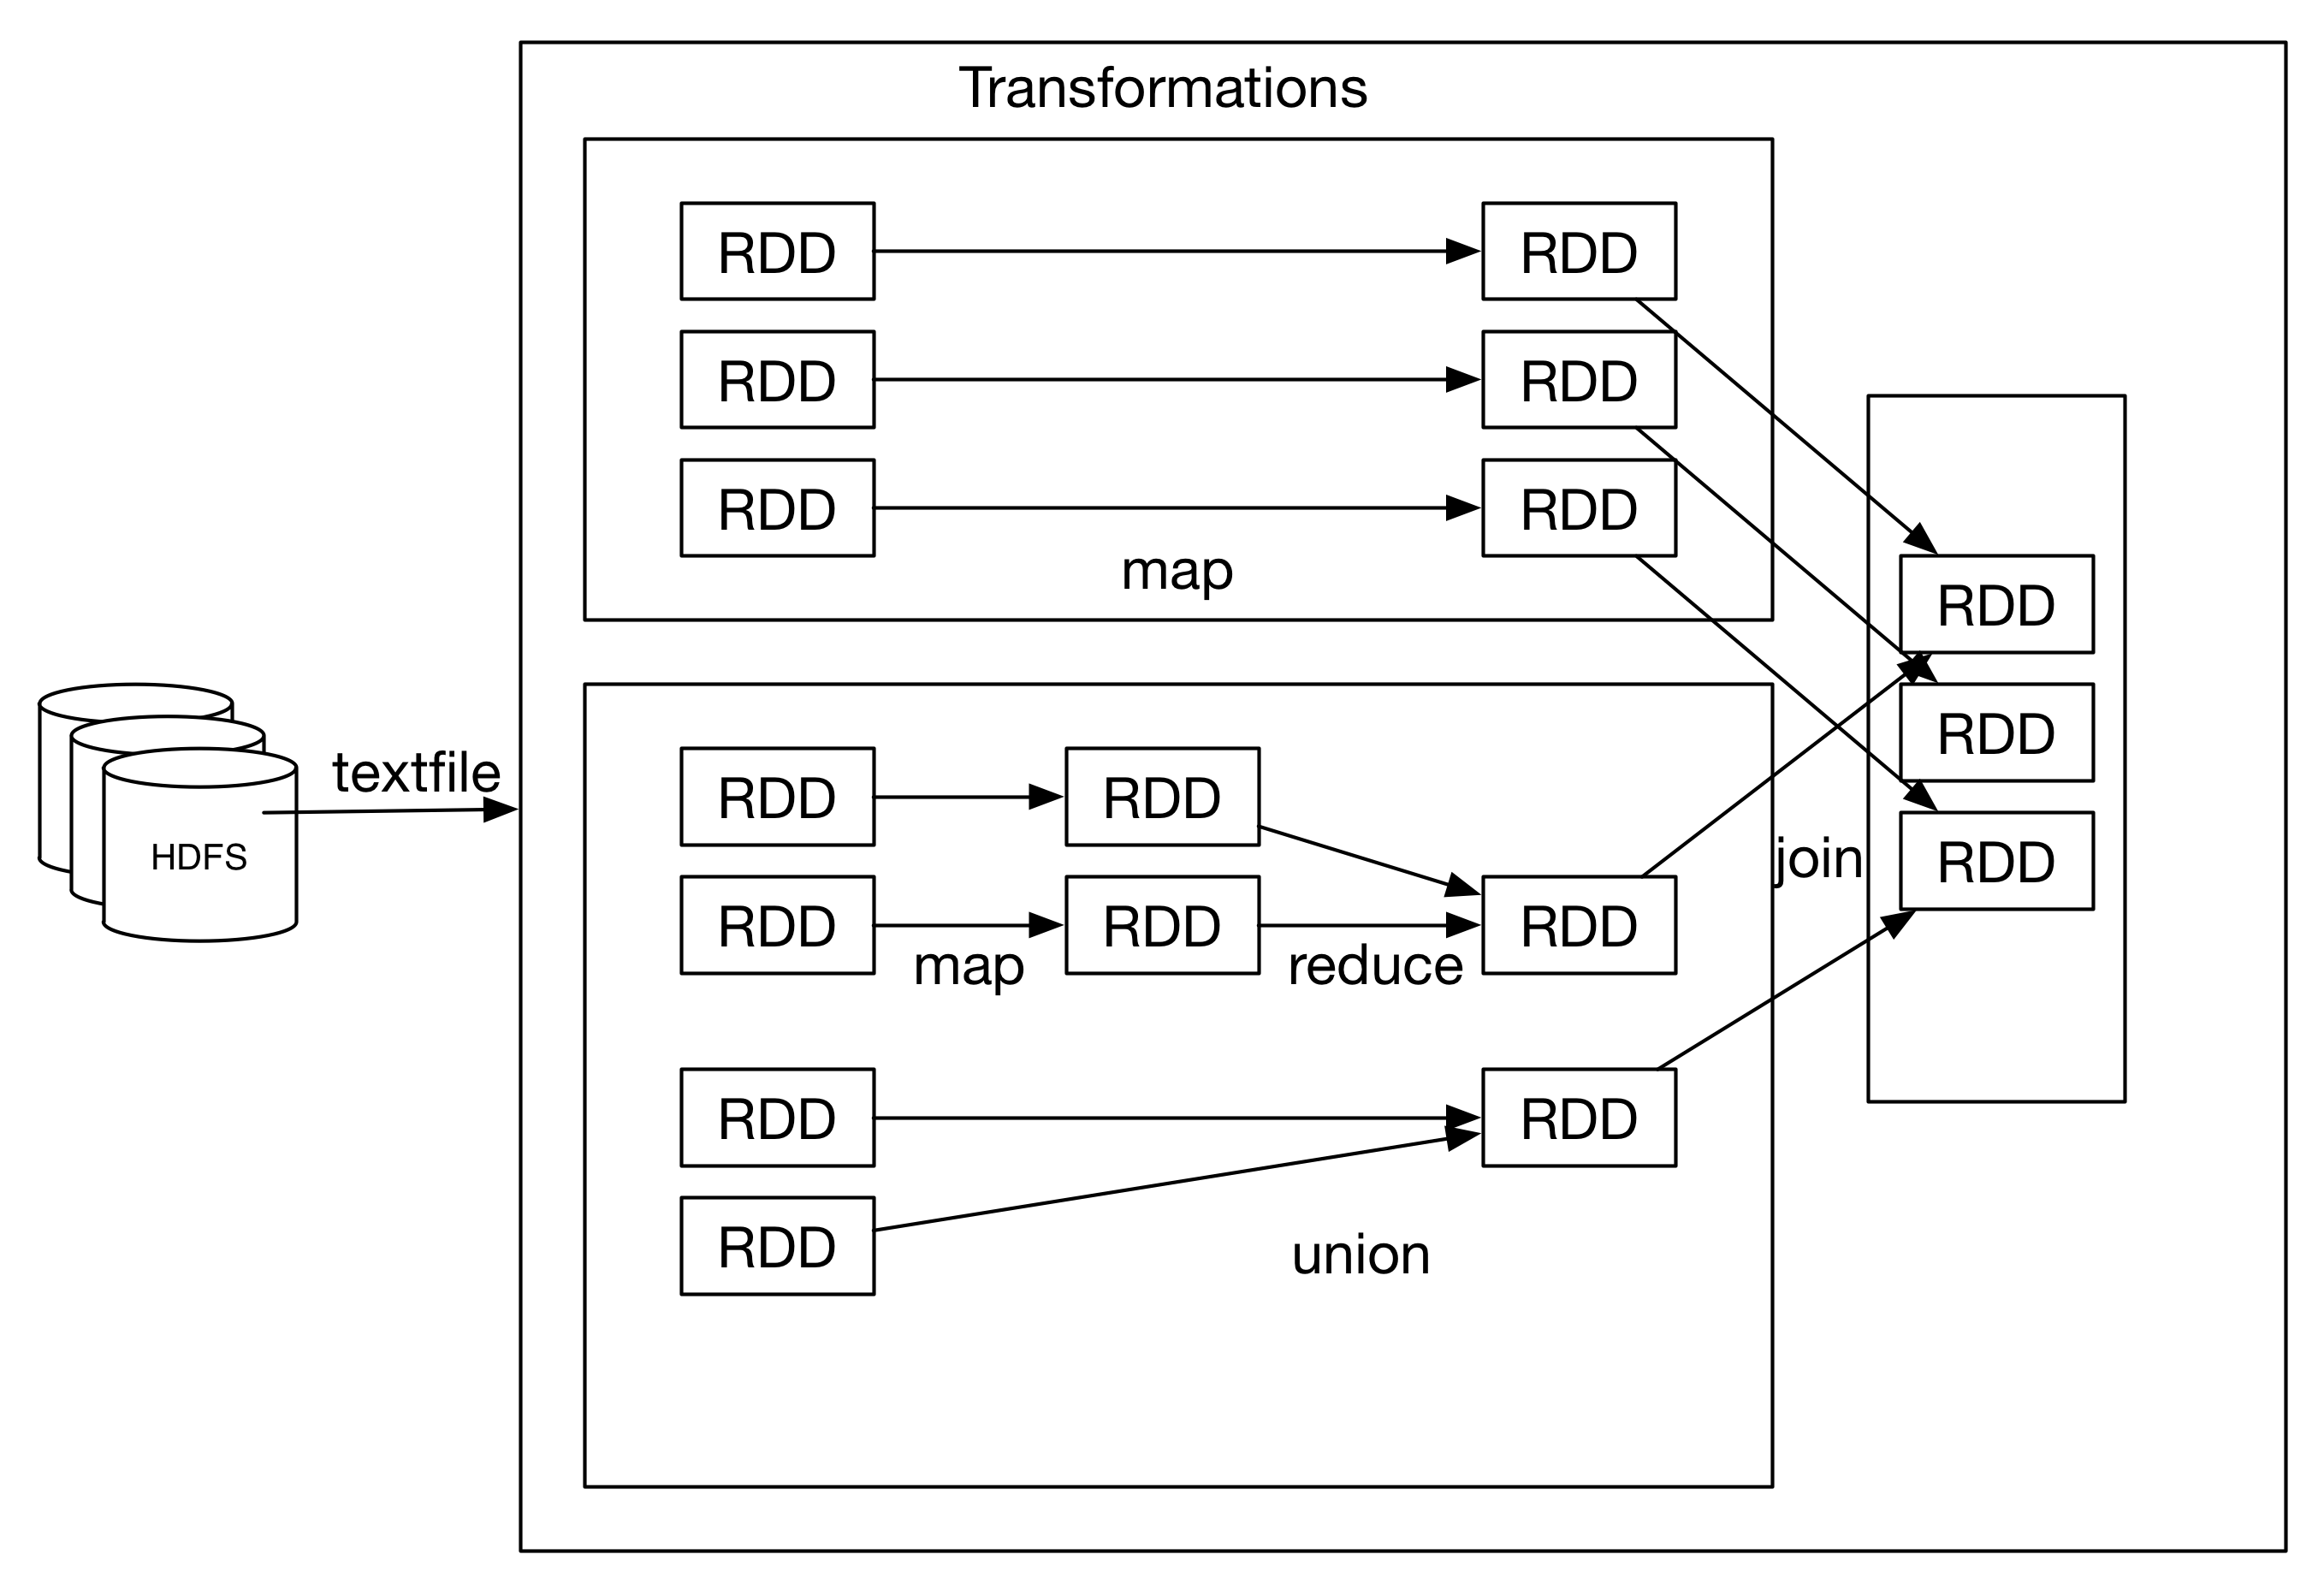
\includegraphics[width=1.0\textwidth]{bilder/rdd_transform.png}
\caption{Schematische Darstellung der Erzeugung und Verarbeitung von RDDs aus persistierten Daten}
\label{fig:rddunkt}
\end{figure}

Im Gegensatz zu den Transformations, die immer ein neues RDD als Ergebnismenge erzeugen, liefern die Actions ein Ergebnis zurück, das entweder an das Driver-Program auf dem Spark Master zurückgegeben, oder im Dateisystem persistiert wird. 

Die Tabelle \ref{tab:actions} zeigt exemplarisch einige wichtige Actions, die auf RDDs angewendet werden können. Eine vollständige Übersicht aller Actions befindet sich im Anhang dieser Arbeit. 


\begin{table}[!ht]
\centering
\begin{tabular}{| p{5cm} | p{8cm} | }
\hline
Actions & Zweck \\ \hline \hline
reduce(func) & Aggregate the elements of the dataset using a function func (which takes two arguments and returns one). The function should be commutative and associative so that it can be computed correctly in parallel.  \\ \hline 
collect() & Return all the elements of the dataset as an array at the driver program. This is usually useful after a filter or other operation that returns a sufficiently small subset of the data. \\ \hline 
count() & Return the number of elements in the dataset. \\ \hline 
first() & Return the first element of the dataset (similar to take(1)). \\ \hline 
\end{tabular}
\caption{Übersicht der einiger wichtiger Actions auf RDDs}
	\label{tab:actions}
\end{table}



Generell kapselt Spark seine Variablen in die jeweiligen Tasks \citeint{adv12}. So kennt jeder Knoten nur die Variablen, die zu dem durch Spark deployten Task gehören. Ist es notwendig, dass große RDDs über Tasks hinweg verfügbar gemacht werden müssen, bietet sich hierfür die Funktion \textit{Broadcast} an. Nach dem Erstellen eines RDD ist es möglich, dem SparkContext mitzuteilen, dass diese erzeugte Collection über Taskgrenzen hinweg verteilt werden soll. 

Folgender Codeausschnitt soll dieses Vorgehen verdeutlichen \citeint{adv12}: 

\begin{lstlisting}[label=broadcast,caption=Verwendung der Broadcast-Variablen in Spark]
val pageNames = sc.textFile(“pages.txt”).map(...)
val pageMap = pageNames.collect().toMap()
val bc = sc.broadcast(pageMap)
val visits = sc.textFile(“visits.txt”).map(...)
val joined = visits.map(v => (v._1, (bc.value(v._1), v._2)))
\end{lstlisting}

In der ersten Zeile wird mittels \texttt{map} aus dem Textfile ein RDD erzeugt, in Zeile zwei wird durch collect eine neue Map erzeugt und die dritte Zeile teilt dem SparkContext mit, dass diese über die Task- und Node-Grenzen hinweg verteilt werden soll. Der Variablen \texttt{joined} wird in Zeile fünf mittels des Aufrufs von \texttt{bc.value} der Wert der geteilten Variable übergeben.



\section{RDD Persistenz: Storage-Level von Spark}
\label{section:storage lvl}

Wie im vorhergehenden Abschnitt erwähnt wurde, lässt sich Spark durch den Anwender eine eigene Definition der Speicherstrategie von Spark zu. Zu diesem Zweck stellt die API von Spark hier sieben verschiedene Storage-Levels  zur Verfügung. Standardmäßig verwaltet Spark die Speicherzuteilung und Lokalisierung der generierten RDDs selbst nach der Prämisse,  diese in der Form zu partitionieren, dass sie möglichst im RAM der jeweiligen Konten Platz finden. Es existieren aber durchaus Nutzungsfälle, wo ein manuelles Eingreifen des Nutzers in diese Strategie sinnvoll ist. 

Im Folgenden werden die Storage-Levels von Spark vorgestellt (aus \citeint{spa15}): 

\begin{itemize}
\item MEMORY\_ONLY	Store RDD as deserialized Java objects in the JVM. If the RDD does not fit in memory, some partitions will not be cached and will be recomputed on the fly each time they're needed. This is the default level.
\item MEMORY\_AND\_DISK	Store RDD as deserialized Java objects in the JVM. If the RDD does not fit in memory, store the partitions that don't fit on disk, and read them from there when they're needed.
\item MEMORY\_ONLY\_SER	Store RDD as serialized Java objects (one byte array per partition). This is generally more space-efficient than deserialized objects, especially when using a fast serializer, but more CPU-intensive to read.
\item MEMORY\_AND\_DISK\_SER	Similar to MEMORY\_ONLY\_SER, but spill partitions that don't fit in memory to disk instead of recomputing them on the fly each time they're needed.
\item DISK\_ONLY	Store the RDD partitions only on disk.
\item MEMORY\_ONLY\_2, MEMORY\_AND\_DISK\_2, etc.	Same as the levels above, but replicate each partition on two cluster nodes.
\item OFF\_HEAP (experimental)	Store RDD in serialized format in Tachyon. Compared to MEMORY\_ONLY\_SER, OFF\_HEAP reduces garbage collection overhead and allows executors to be smaller and to share a pool of memory, making it attractive in environments with large heaps or multiple concurrent applications. Furthermore, as the RDDs reside in Tachyon, the crash of an executor does not lead to losing the in-memory cache. In this mode, the memory in Tachyon is discardable. Thus, Tachyon does not attempt to reconstruct a block that it evicts from memory.

\end{intemize}

Wenn ein RDD problemlos in den Speicher passt, sollte man dessen Level auf der Default-Einstellung MEMORY\_ONLY belassen, da dies die schnellsten Ausführungszeiten garantiert. Ist dies nicht der Fall, sollte die Verwendung MEMORY\_ONLY\_SER in Verbindung mit einem schnellen Serialisierer getestet werden. Generell wird empfohlen, Überläufe der RDDs auf den Festspeicher wenn möglich zu verhindern. Nur wenn die Berechnungsfunktionen zur Erstellung der RDDs sehr teuer waren, oder die Ergebnismenge sehr umfangreich ist, sollte diese Möglichkeit genutzt werden. In diesem Fall ist die Weiterverarbeitungsgeschwindigkeit durch Spark auf die Lesegeschwindigkeit des Festspeichers beschränkt.    


\section{Die Spark-Console REPL}
\label{section:repl}

TBD!



\section{Die Spark APIs}
\label{section:APIs}
TBD!

\subsection{Spark Scala API}
\label{section:scala}

TBD!

\subsection{Spark Java API}
\label{section:java}

TBD!

\subsection{Spark Python API}
\label{section:python}

TBD!

\subsection{Third Level API für Spark mit Clojure: Flambo}
\label{section:flambo}

TBD!

\subsection{Third Level API für Spark mit R: SparkR}
\label{section:sparkr}

TBD!



\section{Zusammenfassung}
\label{section:zusammen}



TBD!






















